\section{What Can Go Wrong?}
\begin{frame}{What Can Go Wrong?}
    Since our task is to select a learning algorithm and train it on data, there are two main sources of failure:
    \vspace{1em}
    \begin{columns}[c]
        \begin{column}{0.50\textwidth}
            \centering
            \begin{tcolorbox}[colback=red!5, colframe=red!60, title=\textbf{1. Bad Data}]
                \begin{itemize}
                    \item Not enough data
                    \item Non-representative data
                    \item Poor quality (Noise)
                    \item Irrelevant features
                \end{itemize}
            \end{tcolorbox}
        \end{column}
        \begin{column}{0.03\textwidth}
            \centering \textbf{+}
        \end{column}
        \begin{column}{0.52\textwidth}
            \centering
            \begin{tcolorbox}[colback=blue!5, colframe=blue!60, title=\textbf{2. Bad Algorithm}]
                \begin{itemize}
                    \item Overfitting
                    \item Underfitting
                \end{itemize}
            \end{tcolorbox}
        \end{column}
    \end{columns}
\end{frame}


% --- SLIDE 1: INSUFFICIENT DATA (The Scale Plot) ---
\begin{frame}{Problem 1: Insufficient Data}

    \begin{columns}[c]
        \begin{column}{0.4\textwidth}
            \textbf{The Reality Gap}
            \vspace{1em}
            \begin{itemize}
                \item \textbf{Humans:} Can generalize from 1 example (Zero-shot).
                \item \textbf{Machines:} Need thousands to find the signal in the noise.
            \end{itemize}
            
            \vspace{1em}
            \small \textit{Without enough data, complex models just memorize the noise.}
        \end{column}

        \begin{column}{0.6\textwidth}
            \centering
            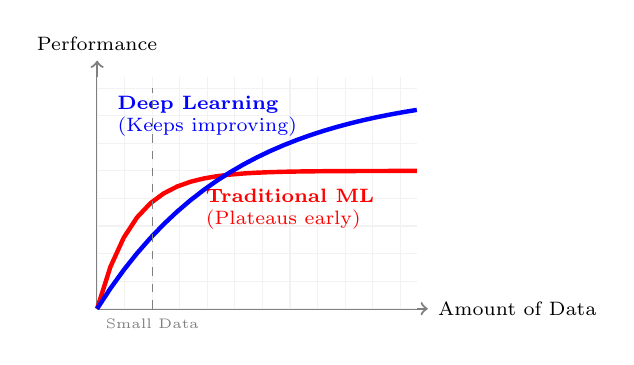
\begin{tikzpicture}[scale=0.7]
                % Axes
                \draw[->, thick, gray] (0,0) -- (6,0) node[right, black] {\scriptsize Amount of Data};
                \draw[->, thick, gray] (0,0) -- (0,4.5) node[above, black] {\scriptsize Performance};
                
                % Grid
                \draw[gray!10, step=0.5] (0,0) grid (5.8,4.2);

                % Traditional ML (Plateau)
                \draw[red, ultra thick, domain=0:5.8] plot (\x, {2.5 * (1 - exp(-1.5*\x))});
                \node[red, align=left, font=\scriptsize] at (3.5, 1.8) {\textbf{Traditional ML}\\(Plateaus early)};
                
                % Deep Learning (Scale)
                \draw[blue, ultra thick, domain=0:5.8] plot (\x, {4.0 * (1 - exp(-0.4*\x))});
                \node[blue, align=left, font=\scriptsize] at (2.0, 3.5) {\textbf{Deep Learning}\\(Keeps improving)};
                
                % Dotted connector
                \draw[dashed, gray] (1, 0) -- (1, 4);
                \node[below, font=\tiny, gray] at (1,0) {Small Data};
            \end{tikzpicture}
        \end{column}
    \end{columns}
\end{frame}

% --- SLIDE 2: SAMPLING BIAS (Text Only) ---
\begin{frame}{Problem 2: Non-Representative Data (Bias)}

    \begin{alertblock}{Definition: Sampling Bias}
        When your training data does not accurately reflect the real world you want to predict.
    \end{alertblock}


    \begin{tcolorbox}[colback=blue!5, colframe=blue!50, title=Example: The "Happiness" Model]
        \textbf{Scenario:}
        \begin{itemize}
            \item You want to predict \textbf{Happiness} based on \textbf{Wealth}.
            \item But you only collect data from the \textbf{Middle Class}.
        \end{itemize}
        
        \vspace{0.5em}
        \textbf{The Result:}
        \begin{itemize}
            \item The model learns: \textit{"More Money = More Happy."}
            \item \textbf{Fail:} It will fail catastrophically for \textbf{Billionaires} (where money stops mattering) or \textbf{Poverty} (where struggles are different).
        \end{itemize}
    \end{tcolorbox}

\end{frame}

\begin{frame}{Problems 3 \& 4: Poor Quality \& Irrelevant Features}
    \begin{columns}[T]
        \begin{column}{0.48\textwidth}
            \textbf{Poor Quality Data}
            \begin{itemize}
                \item \textbf{Noise:} Random errors in the data.
                \item \textbf{Outliers:} Extreme values that distort the pattern.
                \item \textbf{Missing Values:} Empty cells in your spreadsheet.
            \end{itemize}
            \vspace{0.5em}
            \textit{Solution: Data Cleaning (takes ~80\% of a Data Scientist's time).}
        \end{column}
        \begin{column}{0.48\textwidth}
            \textbf{Irrelevant Features}
            \begin{itemize}
                \item \textit{"Garbage In, Garbage Out"}
                \item If you try to predict "Price of a Car" using "Color of the seats", the model will fail.
            \end{itemize}
            \vspace{0.5em}
            \textit{Solution: Feature Engineering (Selection \& Extraction).}
        \end{column}
    \end{columns}
\end{frame}

% --- Subsection: Bad Algorithm ---
\section{Generalization}
\subsection{Overfitting vs. Underfitting}
